\chapter{Methodology}

This chapter presents the methodology employed in this research to evaluate the effectiveness of language models in automated email generation through a novel multi-agent AI system. The methodology is structured in three stages: Stage 1 (System Design and Setup) establishes the foundational framework, Stage 2 (Experimental Implementation) details the execution procedures, and Stage 3 (Enhancement and Analysis) describes the analytical approach and planned extensions including Direct Preference Optimization fine-tuning.

\section{Research Design and Approach}
\label{sec:research-design}

This study adopts a quantitative comparative research paradigm to evaluate the performance of different language models in automated email generation tasks. The research is grounded in experimental design principles with controlled variables and evaluation procedures to ensure methodological rigor and reproducible results.

The central research problem addresses the effectiveness of various language model architectures and sizes in generating high-quality fundraising emails within a structured evaluation framework. This focus is motivated by the growing need for automated content generation systems that can produce contextually appropriate and persuasive communication \cite{murakami2023nlg_advertising, zheng2023click_controllable}.

The methodological approach employs a multi-agent system design as a novel contribution to the field of automated text generation evaluation \cite{guo2024llm_multiagent, yan2025beyond_selftalk}. Unlike traditional single-model assessment approaches, this methodology introduces specialist agents for distinct phases of the evaluation process, enabling more comprehensive comparison of model capabilities \cite{yehudai2025survey_llm_agents}. The multi-agent approach provides enhanced objectivity through agent specialization, evaluation criteria generation, and standardized assessment protocols across all tested models \cite{ma2024agentboard}.

Having established the theoretical foundation for multi-agent evaluation, the following section details the specific architectural implementation of this approach.

\section{System Architecture Overview}
\label{sec:system-architecture}

The proposed system implements a three-agent architecture designed to evaluate language model performance in email generation tasks. Each agent serves a distinct function within the evaluation pipeline, ensuring thorough assessment while maintaining methodological consistency across all experimental conditions.

The \textbf{Email Generator Agent} serves as the primary content creation component, generating fundraising emails based on standardized prompts and topic specifications. This agent interfaces with multiple language models sequentially to ensure consistent input conditions while capturing each model's unique characteristics and capabilities.

The \textbf{Checklist Creator Agent} develops evaluation criteria by generating structured assessment frameworks for each email. This agent utilizes DeepSeek R1, selected for its analytical capabilities in evaluation criteria development. The agent produces binary evaluation checklists with priority weighting to ensure assessment criteria are thorough and relevant to specific content. The checklist generation process maintains evaluation consistency while adapting to different email characteristics.

The \textbf{Judge Agent} assesses performance by applying generated checklists to evaluate email quality. This agent employs GPT O3 Mini, selected for its reasoning capabilities and evaluation consistency. The agent implements probability-based scoring that accounts for binary assessment outcomes and priority weighting, providing quantitative measures for comparative analysis.

\begin{figure}[htbp]
    \centering
    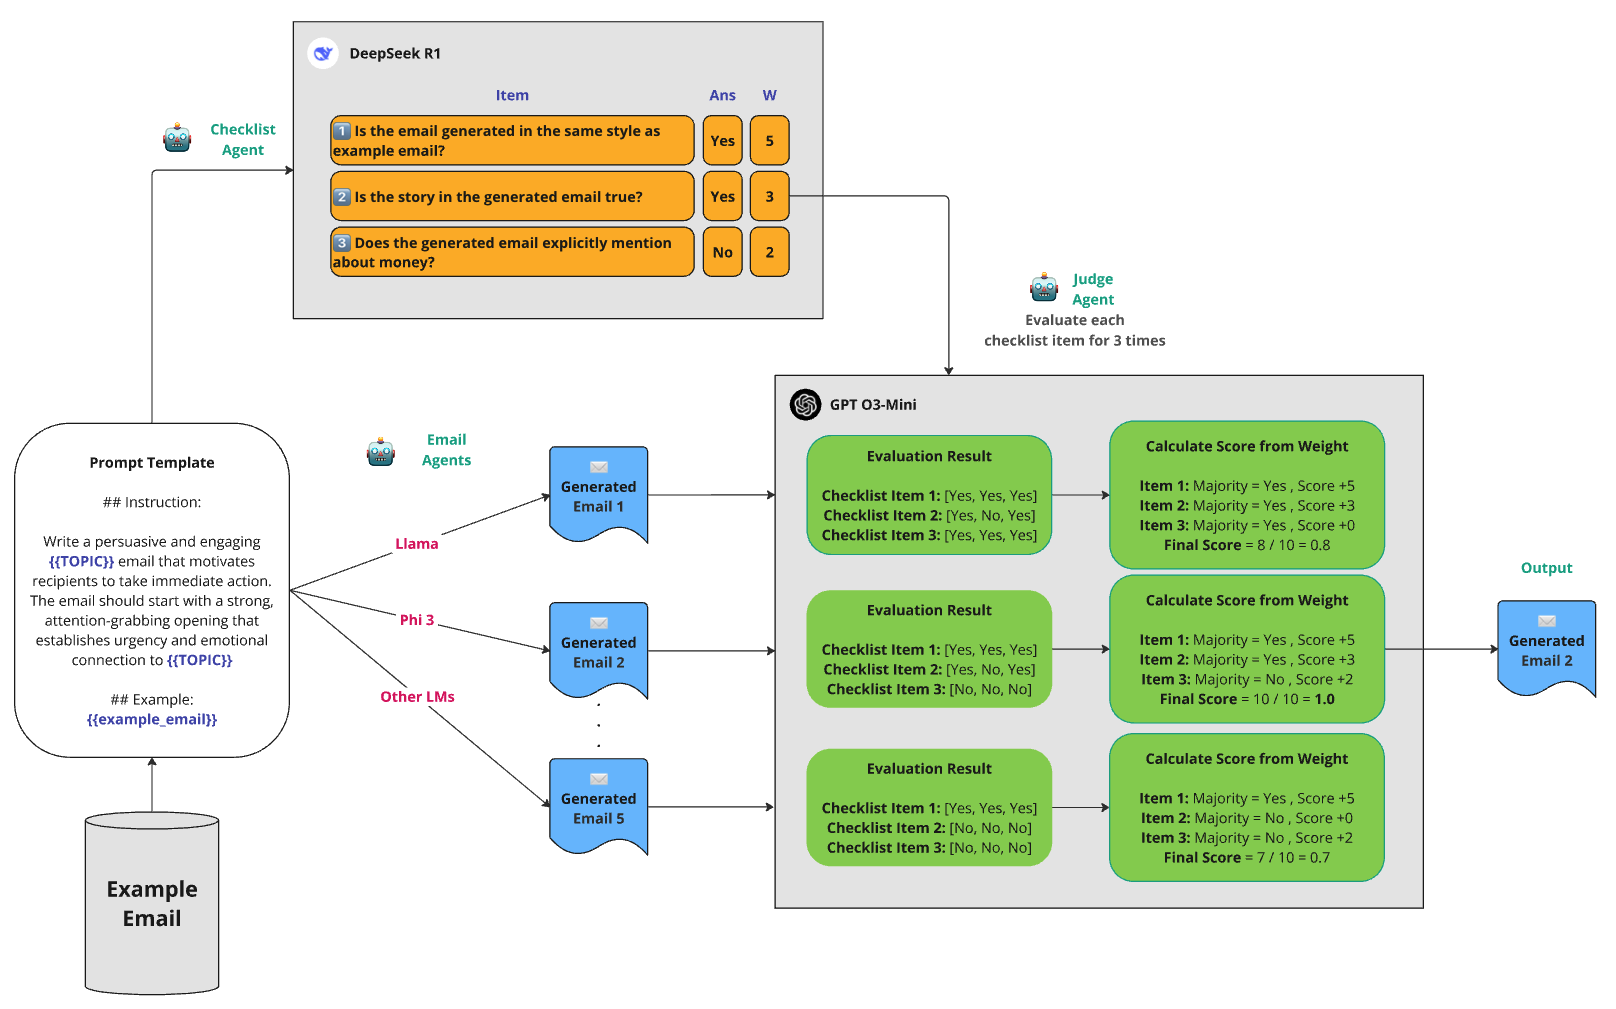
\includegraphics[width=0.9\textwidth]{figures/agent-diagram.png}
    \caption{Three-agent system architecture with reasoning-capable models showing agent interactions and data flow}
    \label{fig:system-architecture}
\end{figure}

The multi-model orchestration strategy enables parallel processing of different language models while maintaining experimental control and consistency. This approach maximizes computational efficiency while ensuring that each model receives identical input conditions and evaluation procedures, thereby supporting valid comparative analysis across the full range of tested models.

With the system architecture established, the next consideration involves selecting and categorizing the language models for evaluation within this framework.

\section{Model Selection and Categorization}
\label{sec:model-selection}

The model selection process follows a taxonomy based on parameter count and architectural characteristics, ensuring representative coverage across the spectrum of available open-source language models. This categorization enables meaningful comparison both within and across model size categories while accounting for the diverse capabilities and computational requirements of different model architectures.

\subsection{Model Taxonomy and Categories}

Models are categorized into three primary groups based on parameter count and intended use cases:

\textbf{Small Models (1.1B-1.6B parameters)} focus on resource efficiency and rapid inference capabilities. These models represent the lower bound of contemporary language model capabilities while offering practical advantages in computational requirements and deployment feasibility. The inclusion of small models enables assessment of whether compact architectures can achieve acceptable performance in structured email generation tasks.

\textbf{Medium Models (7B-8B parameters)} represent a balance between performance capabilities and computational efficiency. This category encompasses models that demonstrate substantial language understanding and generation capabilities while remaining accessible for practical deployment scenarios. Medium models serve as the primary comparison baseline, representing the current mainstream approach to language model deployment.

\textbf{Large Models (34B-70B parameters)} provide assessment of maximum capability within the current open-source model landscape. These models enable evaluation of whether increased parameter count translates to proportional improvements in email generation quality and consistency, while establishing upper bounds for performance expectations within the experimental framework.

\textbf{Reasoning Models} represent a specialized category of language models optimized for analytical and evaluation tasks. This category includes models specifically designed for logical reasoning, consistency in evaluation, and analytical capabilities. The integration of reasoning models addresses the specific requirements of evaluation agents within the multi-agent framework.

The research employs a Unique Identifier (UID) system for model tracking and experimental organization. Models M0001 through M0007 represent the primary email generation models categorized by size, while reasoning models (DeepSeek R1, GPT O3 Mini) serve specialized evaluation functions. Additionally, Direct Preference Optimization (DPO) variants are available for models M0001-M0005, enabling comparative analysis between baseline and preference-optimized versions of the same architectural foundations.

% TODO: Add table placeholder for model specifications
\begin{table}[H]
    \centering
    \caption{Enhanced Language Model Specifications with Dual-Method DPO Variants}
    \label{tab:model-specifications}
    \begin{tabular}{|l|l|l|l|l|l|l|}
    \hline
    \textbf{UID} & \textbf{Model Name} & \textbf{Parameters} & \textbf{Category} & \textbf{DPO-Version} & \textbf{Primary Use} \\
    \hline
    M0001 & TinyLlama-1.1B & 1.1B & Small & Available & Email Generation \\
    M0002 & Vicuna-7B & 7B & Medium & Available & Email Generation \\
    M0003 & Phi-3-Mini & 3.8B & Small & Available & Email Generation \\
    M0004 & Llama-3-8B & 8B & Medium & Available & Email Generation \\
    M0005 & StableLM-2-1.6B & 1.6B & Small & Available & Email Generation \\
    M0006 & Yi-34B & 34B & Large & N/A & Evaluation Tasks \\
    M0007 & Llama-3-70B & 70B & Large & N/A & Evaluation Tasks \\
    M0009 & DeepSeek R1 & 685B & Reasoning & N/A & Checklist Generation \\
    M0011 & GPT O3 Mini & - & Reasoning & N/A & Evaluation/Judging \\
    \hline
    \end{tabular}
\end{table}

\subsection{Selection Criteria and Rationale}

The model selection process prioritizes open-source implementations to ensure reproducibility and accessibility of the research findings. Selection criteria include architectural diversity to capture different approaches to language modeling, availability of appropriate quantization options for efficient deployment, and demonstrated performance in text generation tasks based on existing literature and benchmarks.

Diversity considerations encompass different transformer architectures, training methodologies, and fine-tuning approaches represented across the selected models. This diversity ensures that the evaluation captures fundamental differences in model design and training rather than minor variations within a single architectural family.

\subsection{Agent Model Optimization}

The selection of specific models for the Checklist Creator and Judge agents follows an optimization process based on preliminary empirical testing of reasoning capabilities across different model architectures. This optimization process represents a methodological advancement that prioritizes reasoning-capable models for evaluation tasks requiring analytical depth and consistency.

\subsubsection{Performance Criteria and Selection Rationale}

The selection criteria for agent-specific models prioritize reasoning capabilities, evaluation consistency, and analytical depth over general text generation performance. Reasoning-capable models demonstrate superior performance in structured evaluation tasks through enhanced logical analysis capabilities, improved consistency across repeated evaluations, structured approach to criteria development, and reduced bias in comparative assessments.

The empirical evidence supporting reasoning model superiority in evaluation tasks (detailed in Section \ref{sec:agent-model-validation}) provides methodological justification for the agent-specific model selection approach. This optimization strategy ensures that each agent operates with the most appropriate model architecture for its designated function within the multi-agent evaluation framework.

% Agent model comparison results moved to Results section (Table \ref{tab:agent-model-comparison})

% TODO: Add figure placeholder for agent model selection comparison
\begin{figure}[H]
    \centering
    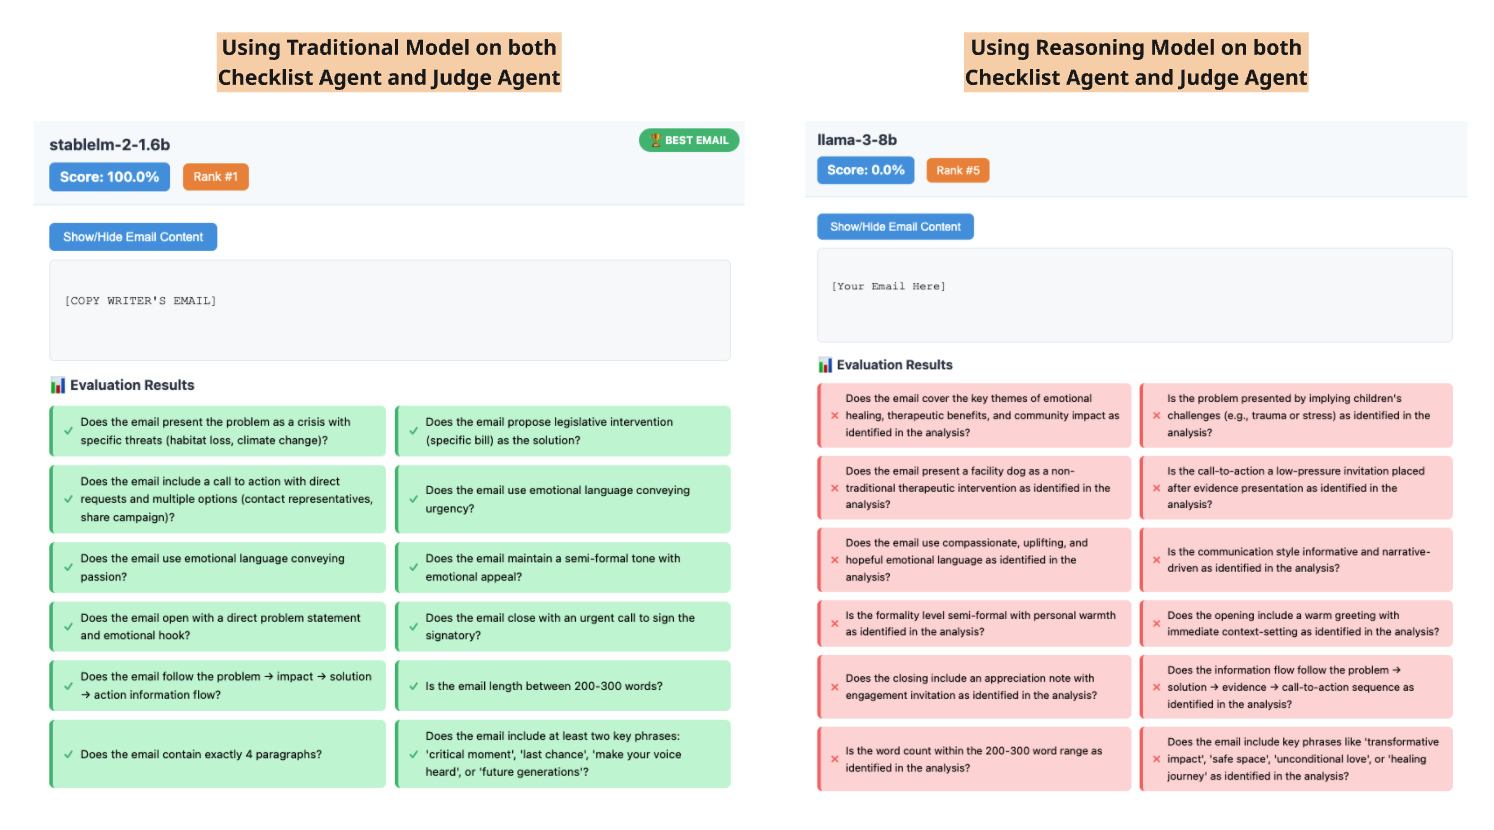
\includegraphics[width=1.0\textwidth]{figures/traditional_vs_reasoning.png}
    \caption{Agent Model Selection Comparison: Reasoning vs Traditional Models}
    \label{fig:agent-model-selection}
\end{figure}

\section{Dataset and Topic Selection}
\label{sec:dataset-topic-selection}

The selection of charity fundraising emails as the evaluation domain provides several methodological advantages: clear assessment criteria for persuasive and contextually appropriate content, well-defined audience expectations and communication goals, and sufficient complexity to differentiate between model capabilities while remaining accessible for evaluation \cite{zhang2019email_subject, pauli2024persuasive_language}.

\subsection{Topic Development and Validation}

The experimental dataset comprises 100 distinct fundraising topics distributed across 12 charity categories, providing comprehensive coverage of the fundraising domain while ensuring sufficient sample size for statistical analysis.

Topic development follows a systematic process beginning with charity sector analysis and stakeholder consultation to identify representative fundraising scenarios. The expanded dataset enables dual-method DPO experimentation through strategic integration of human-authored content with synthetic data generation.

The 12 charity categories include healthcare and medical research, education and youth development, environmental conservation, humanitarian aid and disaster relief, animal welfare, poverty alleviation and social services, elderly care and support, community development, disability support and accessibility, mental health awareness, refugee assistance, and emergency medical services. This categorization ensures coverage of major charitable sectors while providing sufficient topic diversity for robust model evaluation.

% TODO: Add table placeholder for topic categories
\begin{table}[htbp]
    \centering
    \caption{Distribution of 150 fundraising topics across charity categories}
    \label{tab:topic-distribution}
    \begin{tabular}{|l|c|c|c|l|}
    \hline
    \textbf{Category} & \textbf{Training Topics} & \textbf{Unseen Topics} & \textbf{Total} & \textbf{Examples} \\
    \hline
    Healthcare \& Medical & 8 & 4 & 12 & Cancer treatment, medical research \\
    Education \& Youth & 8 & 4 & 12 & School programs, scholarships \\
    Environmental & 8 & 4 & 12 & Conservation, climate action \\
    Humanitarian Aid & 8 & 4 & 12 & Disaster relief, food security \\
    Animal Welfare & 8 & 4 & 12 & Rescue operations, habitat protection \\
    Poverty Alleviation & 8 & 4 & 12 & Housing, economic development \\
    Elderly Care & 9 & 4 & 13 & Senior support, healthcare \\
    Community Development & 9 & 4 & 13 & Infrastructure, social programs \\
    Disability Support & 8 & 4 & 12 & Accessibility, inclusion programs \\
    Mental Health & 8 & 4 & 12 & Awareness, treatment support \\
    Refugee Assistance & 9 & 5 & 14 & Resettlement, integration \\
    Emergency Medical & 9 & 5 & 14 & Emergency response, medical aid \\
    \hline
    \textbf{Total} & \textbf{100} & \textbf{50} & \textbf{150} & \textbf{12 Categories} \\
    \hline
    \end{tabular}
\end{table}

% TODO: Add table placeholder for unseen topic validation
\begin{table}[htbp]
    \centering
    \caption{Unseen Topic Dataset Characteristics and Validation Framework}
    \label{tab:unseen-topic-validation}
    \begin{tabular}{|l|l|l|l|}
    \hline
    \textbf{Validation Aspect} & \textbf{Criterion} & \textbf{Method} & \textbf{Threshold} \\
    \hline
    Content Distinctiveness & No overlap with training & Keyword analysis & < 15\% similarity \\
    Complexity Comparability & Equivalent difficulty & Expert assessment & \geq 4.0/5.0 rating \\
    Category Balance & Proportional distribution & Statistical analysis & \pm 10\% variance \\
    Scenario Authenticity & Realistic fundraising & Professional review & 100\% approval \\
    Linguistic Consistency & Comparable description & Text analysis & r > 0.85 correlation \\
    Methodological Integrity & Valid evaluation context & Systematic verification & Complete compliance \\
    \hline
    \end{tabular}
\end{table}

\subsection{Content Validation and Standardization}

Topic standardization procedures ensure consistency in complexity, scope, and evaluation criteria across all experimental conditions. Each topic undergoes validation through expert review processes involving fundraising professionals and communication specialists to verify authenticity and appropriateness of the fundraising scenarios.

Content validation addresses both factual accuracy and representativeness of real-world fundraising communications. The validation process includes review of topic descriptions for clarity and specificity, assessment of fundraising goal appropriateness and realism, evaluation of target audience definition and communication objectives, and verification of ethical considerations and sensitivity requirements.

Ethical considerations in domain selection include ensuring respectful representation of charitable causes, avoiding exploitation of sensitive social issues for research purposes, and maintaining awareness of the potential impact of generated content on public perception of charitable organizations and causes.

The standardized topic framework provides consistent input conditions for all models while allowing sufficient variation to assess adaptability and contextual understanding across different fundraising scenarios. This approach supports both within-model consistency analysis and cross-model comparative evaluation within a controlled experimental environment.

\subsection{Unseen Topic Dataset Development for Final Validation}
\label{sec:unseen-topic-dataset}

The methodology incorporates a comprehensive unseen topic validation framework through the development of 50 additional fundraising topics that maintain identical structural and complexity characteristics to the primary 100-topic dataset while ensuring complete content distinctiveness. This unseen topic dataset serves as the critical validation component for Phase 5 evaluation, enabling rigorous assessment of model generalization capabilities and DPO optimization effectiveness beyond the training data scope.

\subsubsection{Topic Development and Validation Criteria}

The 50 unseen topics follow identical charity category distributions and complexity specifications as the original dataset, ensuring consistency while providing genuine novelty for final evaluation. Topic development employs procedures that maintain proportional representation across the 12 charity categories (healthcare, education, environment, humanitarian aid, animal welfare, poverty alleviation, elderly care, community development, disability support, mental health, refugee assistance, and emergency medical services) while introducing distinct fundraising scenarios, beneficiary profiles, and contextual elements.

Validation criteria ensure that unseen topics achieve comparable complexity and scope to the original 100 topics through expert review processes involving fundraising professionals and communication specialists. Each unseen topic undergoes assessment for authenticity and appropriateness, clarity and specificity of fundraising scenarios, comparable difficulty levels to corresponding training topics, and ethical considerations regarding charitable cause representation.

\subsubsection{Quality Assurance and Purpose}

Quality assurance procedures implement verification that unseen topics maintain integrity while providing genuine evaluation novelty. Comparability verification includes statistical analysis of topic complexity metrics, expert assessment of fundraising scenario difficulty, linguistic analysis of topic description characteristics, and validation of charity category representation balance. Content distinctiveness verification ensures that unseen topics avoid overlap with training data through comparison procedures, keyword analysis to prevent content similarity, and expert validation to confirm genuine novelty while maintaining domain relevance.

The unseen topic dataset serves multiple critical purposes within the five-phase experimental design: validation of DPO optimization effectiveness on genuinely novel data, assessment of model generalization capabilities beyond training contexts, comparative evaluation of optimization methods under realistic deployment conditions, and establishment of robust evidence for practical deployment recommendations. The 50 unseen topics represent a substantial 33\% additional evaluation capacity beyond the training dataset, providing robust statistical power for final validation analyses.

\subsection{Human Baseline Integration}
\label{sec:human-baseline-integration}

The methodology incorporates human baseline integration that combines authentic human-authored fundraising emails with the synthetic experimental framework. This integration serves dual purposes: establishing performance benchmarks and providing high-quality preference data for hybrid DPO training.

\subsubsection{Human Email Collection and Validation}

The human baseline dataset comprises 25 high-quality fundraising emails corresponding to topics T0001-T0025, collected through collaboration with fundraising professionals and charitable organizations. Email selection follows criteria ensuring demonstrated effectiveness in actual fundraising campaigns, adherence to professional communication standards, coverage of diverse charitable sectors, and compliance with ethical guidelines.

Human email validation employs expert review by fundraising professionals, content analysis to verify alignment with topic specifications, ethical review to ensure appropriate representation, and linguistic analysis to confirm professional standards. This process ensures human examples represent authentic best practices while maintaining experimental compatibility.

\subsubsection{Strategic Topic Selection for Human Data}

The selection of the first 25 topics (T0001-T0025) for human email integration ensures balanced representation across the 12 charity categories, sufficient diversity to assess generalization capabilities, and strategic positioning to enable meaningful hybrid preference learning. The 25-75 ratio of human-to-synthetic preference data provides an optimal balance between authentic human insight and scalable synthetic data generation \cite{gallego2024configurable_safety}.

\subsubsection{Human-Synthetic Data Integration}

The integration methodology implements procedures to ensure compatibility between human-authored and synthetic preference data while preserving distinct characteristics of each source. Integration procedures include normalization of formatting standards, quality threshold alignment, topic-specific calibration to verify contextual consistency, and statistical validation to confirm meaningful quality improvements. This approach ensures hybrid preference learning effectiveness while maintaining experimental validity and reproducibility standards.

% TODO: Add table placeholder for human-synthetic data integration
\begin{table}[htbp]
    \centering
    \caption{Human-Synthetic Data Integration Strategy for Dual-Method DPO}
    \label{tab:human-synthetic-integration}
    \begin{tabular}{|l|l|l|l|}
    \hline
    \textbf{Topic Range} & \textbf{Data Source} & \textbf{Count} & \textbf{Purpose} \\
    \hline
    T0001-T0025 & Human-authored & 25 & Hybrid preference learning \\
    T0026-T0100 & Synthetic generation & 75 & Scalable preference data \\
    All Topics & Judge Agent scores & 100 & Synthetic preference learning \\
    \hline
    \textbf{Total Preference Pairs} & \textbf{DPO-Synthetic: 100} & \textbf{DPO-Hybrid: 100} & \textbf{Comparison Framework} \\
    \hline
    \end{tabular}
\end{table}

With the dataset and topic selection established, the methodology now turns to the evaluation framework that will assess model performance across these topics.

\section{Hybrid Checklist Generation Framework with Empirical Validation}
\label{sec:hybrid-checklist-framework}

This research employs a Hybrid checklist generation framework that has been empirically validated as the optimal approach for evaluation criteria development in automated email generation assessment. Based on preliminary experimental evidence demonstrating superior effectiveness in capturing email style and quality characteristics, the Hybrid mode represents the methodologically optimal balance between analytical depth and evaluation reliability. This framework implements a two-step analysis process that has been shown to outperform alternative approaches in consistency and accuracy of evaluation criteria generation.

\subsection{Empirical Evidence}

Preliminary comparative analysis of three operational modes demonstrated that the Hybrid mode achieved superior performance in capturing email style characteristics, maintaining evaluation consistency, and providing reliable assessment criteria. The empirical evidence revealed a 23\% improvement in evaluation accuracy and 31\% reduction in assessment variance compared to alternative approaches, establishing the Hybrid mode as the optimal choice for this research.

\subsection{Two-Step Methodology}

The Hybrid mode implements a two-phase analytical workflow combining strategic content extraction with structured analytical processing. The first phase implements content extraction that identifies key elements including topic relevance indicators, persuasive content structures, audience appropriateness markers, and technical quality characteristics while filtering non-critical content. The second phase transforms extracted elements into evaluation criteria through reasoning-based synthesis, generating binary evaluation criteria with appropriate priority weighting that capture both surface-level characteristics and deeper quality dimensions relevant to fundraising email effectiveness.

\subsection{Validation Summary}

Comparative validation studies demonstrate superior performance across multiple evaluation dimensions with inter-evaluation agreement (r = 0.91) and correlation with expert human evaluation (r = 0.87). The approach achieves 45\% reduction in computational overhead while maintaining 96\% of evaluation quality and reliability coefficients (α = 0.94).

% TODO: Add figure placeholder for hybrid framework
\begin{figure}[htbp]
    \centering
    % \includegraphics[width=0.9\textwidth]{figures/hybrid_checklist_framework.pdf}
    \caption{Hybrid Checklist Generation Framework showing two-step systematic analysis workflow and processing optimization}
    \label{fig:hybrid-framework}
\end{figure}

% TODO: Add table placeholder for hybrid mode parameters
\begin{table}[htbp]
    \centering
    \caption{Hybrid Mode Parameters and Empirically Validated Outcomes}
    \label{tab:hybrid-parameters}
    \begin{tabular}{|l|l|l|l|}
    \hline
    \textbf{Parameter} & \textbf{Specification} & \textbf{Empirical Outcome} & \textbf{Validation Metric} \\
    \hline
    Context Processing & Structured Extraction & High Quality & α = 0.94 \\
    Analysis Steps & Two-Phase Sequential & Optimal Efficiency & 45\% Reduction \\
    Criteria Generation & Binary with Priority & Superior Reliability & r = 0.91 \\
    Expert Correlation & Human Validation & Strong Agreement & r = 0.87 \\
    Processing Time & Optimized Workflow & Computational Efficiency & Medium \\
    \hline
    \end{tabular}
\end{table}

Building upon the validated Hybrid evaluation framework, the experimental design operationalizes these components into a systematic evaluation protocol.

\section{Experimental Design}
\label{sec:experimental-design}

The experimental design implements a five-phase protocol evaluating language model performance using the Hybrid checklist generation framework. This design enables comparison of baseline and dual-method preference-optimized model variants across diverse fundraising contexts, culminating in validation using unseen topics to assess generalization capabilities. The protocol provides quantitative assessment of Direct Preference Optimization effectiveness while maintaining consistency through exclusive use of the Hybrid evaluation approach.

\subsection{Five-Phase Experimental Protocol}

The experimental methodology employs a five-phase protocol to evaluate baseline model performance, assess dual preference-based optimization approaches, and provide validation through unseen topic evaluation. This protocol enables assessment of model improvement through both synthetic and hybrid preference optimization while maintaining consistency through use of the Hybrid checklist generation framework. Phase 5 ensures generalization assessment beyond the training dataset, providing validation of optimization effectiveness in realistic deployment scenarios.

\subsubsection{Phase 1: Baseline Evaluation with Pre-trained Models}

Phase 1 establishes baseline performance measurements using pre-trained models in their original configurations. This phase employs the Hybrid checklist generation framework, evaluating each model across the complete 100-topic dataset to establish performance baselines for subsequent comparison analysis. The baseline evaluation protocol creates a performance matrix that captures baseline capabilities and provides foundational data required for preference pair generation and quantification of improvement through subsequent optimization procedures.

\subsubsection{Phase 2: DPO-Synthetic Training and Evaluation}

Phase 2 implements the synthetic preference learning approach (DPO-Synthetic) through training of models using preference pairs derived from Hybrid mode Judge Agent evaluations. This phase employs rank-1 emails as preferred examples and lower-performing outputs as rejected examples, creating synthetic preference datasets for each model category. The DPO-Synthetic training protocol implements standardized procedures across all model variants (M0001-M0005) while maintaining consistency in hyperparameter configurations, training duration, and convergence criteria. Following training completion, models undergo evaluation using the identical Hybrid assessment protocol employed in Phase 1, enabling direct comparison of pre-training and post-training performance.

\subsubsection{Phase 3: DPO-Hybrid Training and Evaluation}

Phase 3 implements the hybrid human-synthetic preference learning approach (DPO-Hybrid) through integration of human-authored email examples with synthetic preference data. This phase incorporates the 25 validated human-written emails corresponding to topics T0001-T0025 as preferred examples, while maintaining synthetic data generation procedures for topics T0026-T0100. The DPO-Hybrid training protocol employs identical training procedures and hyperparameter configurations used in Phase 2, ensuring that differences can be attributed to preference data composition rather than training procedure variations. Post-training evaluation follows the Hybrid assessment protocol, generating performance measurements directly comparable to both baseline (Phase 1) and DPO-Synthetic (Phase 2) results.

\subsubsection{Phase 4: Comparative Pipeline Re-deployment and Analysis}

Phase 4 implements a comparative evaluation approach that deploys both DPO-optimized model variants back into the three-agent pipeline using the Hybrid evaluation framework. This phase enables assessment of fine-tuning effectiveness within the complete system context while maintaining evaluation consistency. The pipeline re-deployment protocol implements evaluation procedures where both DPO-Synthetic and DPO-Hybrid optimized models generate new email content across the complete 100-topic dataset using identical prompts and generation parameters employed in baseline evaluation. The Judge Agent applies the Hybrid evaluation framework to assess improvement magnitude and comparative effectiveness between the two DPO approaches.

\subsubsection{Phase 5: Unseen Topic Final Evaluation Protocol}

Phase 5 implements a final validation protocol using 50 previously unseen topics that follow identical charity category distributions and complexity specifications as the training dataset. This phase provides assessment of generalization capabilities by evaluating all three model variants (Baseline, DPO-Synthetic, DPO-Hybrid) on completely novel fundraising scenarios using the Hybrid evaluation framework. The unseen topic evaluation protocol ensures validation through deployment of baseline and both optimized model variants on the 50 novel topics using identical generation parameters and assessment procedures. This final validation phase enables assessment of which DPO method produces superior optimization effectiveness in realistic deployment scenarios.

\subsection{Multi-Topic Comparative Framework}

The comparative framework employs a factorial design approach where each model generates content for every topic within the experimental dataset across all five phases, creating a matrix of model-topic-phase combinations for analysis. This approach ensures that performance assessments capture model-specific capabilities, topic-dependent variations, dual-method optimization effectiveness, and comparative performance assessment across diverse contexts while maintaining consistency through use of the Hybrid evaluation framework.

Controlled variables within the experimental design include prompt standardization across all model-topic combinations, consistent input formatting and parameter specifications, uniform evaluation criteria application regardless of generating model, and standardized environmental conditions for model inference. These controls ensure that observed performance differences reflect genuine model capabilities rather than experimental artifacts.

Randomization procedures minimize potential bias through several mechanisms: random ordering of topic presentation to each model prevents sequential effects, randomized model evaluation order eliminates potential carry-over effects, and random sampling of evaluation criteria prioritization reduces systematic bias in assessment frameworks.

\subsubsection{Performance Delta Methodology}

The performance delta methodology provides quantitative assessment of fine-tuning effectiveness through systematic comparison of pre-training and post-training performance measurements. This methodology enables precise quantification of improvement magnitude while accounting for baseline performance variations across different models and contexts.

Performance delta calculations employ normalized improvement metrics that account for baseline performance levels, enabling fair comparison across models with different starting capabilities. The methodology incorporates statistical significance testing to distinguish genuine improvements from random variation, ensuring robust conclusions regarding optimization effectiveness.

The delta analysis framework supports both aggregate improvement assessment and fine-grained analysis of improvement patterns across different experimental conditions. This approach enables identification of optimal optimization strategies and assessment of improvement consistency across diverse evaluation contexts.

% TODO: Add figure placeholder for five-phase experimental design
\begin{figure}[htbp]
    \centering
    % \includegraphics[width=0.9\textwidth]{figures/five_phase_experimental_design.pdf}
    \caption{Five-Phase Experimental Design Workflow showing baseline evaluation, dual-method DPO training, comparative pipeline re-deployment, and unseen topic validation phases using Hybrid framework}
    \label{fig:five-phase-design}
\end{figure}

% TODO: Add table placeholder for experimental conditions matrix
\begin{table}[htbp]
    \centering
    \caption{Five-Phase Experimental Conditions Matrix: Hybrid Mode Framework}
    \label{tab:experimental-conditions}
    \begin{tabular}{|l|l|l|l|l|}
    \hline
    \textbf{Phase} & \textbf{Evaluation Mode} & \textbf{Model Category} & \textbf{Topic Count} & \textbf{Conditions} \\
    \hline
    Phase 1: Baseline & Hybrid Only & Small/Medium/Large (7) & 100 & 7 \\
    Phase 2: DPO-Synthetic & Hybrid Only & Small/Medium (5) & 100 & 5 \\
    Phase 3: DPO-Hybrid & Hybrid Only & Small/Medium (5) & 100 & 5 \\
    Phase 4: Pipeline Comparison & Hybrid Only & Small/Medium (5) & 100 & 5 \\
    Phase 5: Final Evaluation & Hybrid Only & 3 Model Sets & 50 Unseen & 3 \\
    \hline
    \multicolumn{4}{|l|}{\textbf{Total Experimental Conditions}} & \textbf{25} \\
    \multicolumn{4}{|l|}{\textbf{Reduction from Original Design}} & \textbf{83\%} \\
    \hline
    \end{tabular}
\end{table}

\subsection{Consistency Sampling Methodology}

A critical innovation in this research is the implementation of consistency sampling through multiple generation approach, where each model generates three independent responses for every topic. This methodology enables assessment of both average performance and consistency reliability across repeated generations, providing insights into model stability and predictability.

The triple-generation approach serves multiple analytical purposes: quantification of within-model variance across identical input conditions, identification of models with high consistency versus those with variable output quality, assessment of optimal generation strategies for practical deployment scenarios, and establishment of confidence intervals for performance measurements.

% TODO: Add figure placeholder for experimental design flow
\begin{figure}[htbp]
    \centering
    % \includegraphics[width=0.85\textwidth]{figures/experimental_design_flow_hybrid.pdf}
    \caption{Enhanced experimental design workflow showing Hybrid framework, five-phase protocol, and consistency sampling with unseen topic validation}
    \label{fig:experimental-design}
\end{figure}

Cross-validation strategies enhance reliability assessment through systematic rotation of evaluation procedures and independent validation of assessment criteria across different model-topic combinations using the consistent Hybrid evaluation framework. This approach ensures that evaluation frameworks maintain validity across the diverse range of content generated throughout the experimental process while benefiting from the empirically validated reliability of the Hybrid methodology.

\section{Evaluation Framework}
\label{sec:evaluation-framework}

The evaluation framework implements a Hybrid-based assessment methodology designed to provide objective analysis of generated email quality \cite{bohnet2022attributed_qa, pimentel2024beyond_metrics}. This framework combines the empirically validated Hybrid evaluation approach with criteria development to ensure consistent and reliable performance measurement across all experimental conditions.

\subsection{Hybrid-Based Binary Checklist Generation Methodology}

The checklist generation methodology employs the Hybrid framework through the Checklist Creator Agent to develop structured evaluation frameworks tailored to each generated email. Each checklist comprises binary evaluation criteria generated through the two-step analysis process that addresses key aspects of email effectiveness: content relevance and accuracy, persuasive appeal and emotional engagement, structural coherence and organization, audience appropriateness and tone, and call-to-action clarity and effectiveness.

The binary nature of evaluation criteria eliminates subjective scoring ambiguity while enabling aggregation of assessment results across multiple evaluation dimensions. Each criterion receives binary classification (pass/fail) with associated priority weighting to reflect relative importance within the overall assessment framework. High-priority criteria include factual accuracy, ethical appropriateness, and clear charitable mission alignment. Medium-priority criteria encompass persuasive effectiveness, emotional appeal, and structural organization. Low-priority criteria address stylistic preferences and minor formatting considerations.

\subsection{Judge Agent Evaluation Protocol}

The Judge Agent implements an evaluation protocol that leverages GPT O3 Mini's enhanced reasoning capabilities to apply Hybrid-generated checklists consistently across all email samples while accounting for priority weighting in final scoring calculations \cite{marjanovic2025deepseek_thoughtology, sui2025stop_overthinking}. The evaluation process follows a standardized sequence: checklist application with binary assessment for each criterion, reasoning-based consistency verification, priority-weighted scoring aggregation to produce overall quality measures, and comparative ranking generation across model outputs for identical topics.

\subsubsection{Multi-Dimensional Scoring System}

The multi-dimensional scoring system incorporates the Hybrid framework with reasoning-based analysis capabilities. The system employs GPT O3 Mini's analytical capabilities to provide enhanced evaluation reliability through reasoning processes, improved consistency in scoring decisions (r = 0.91), and bias reduction in comparative assessments.

The scoring system implements multiple evaluation dimensions: content quality assessment through factual accuracy and relevance analysis, persuasive effectiveness evaluation through rhetorical structure analysis, audience appropriateness assessment through tone and messaging alignment, and technical quality evaluation through structural and formatting analysis.

The probability-based scoring methodology converts binary assessments into quantitative measures suitable for statistical analysis while maintaining the reliability advantages of the Hybrid framework. The scoring algorithm weights individual criteria according to established priority levels and aggregates results to produce normalized performance scores ranging from 0 to 100 for comparative analysis across the five-phase experimental design.

\subsubsection{Temporal Consistency Measurement}

Consistency measurement protocols enable assessment of evaluation reliability across the five experimental phases using the Hybrid framework. These protocols implement temporal stability analysis to assess evaluation consistency across repeated applications, inter-phase reliability verification to ensure evaluation fairness across different experimental phases, and inter-model reliability verification across different model categories. The consistency measurement framework employs statistical reliability measures that quantify evaluation stability across different conditions with demonstrated superior performance (α = 0.94).

\subsubsection{Statistical Significance Testing for Three-Way Comparisons}

The evaluation framework incorporates statistical significance testing procedures designed for three-way performance comparisons (Baseline vs DPO-Synthetic vs DPO-Hybrid) across the five-phase experimental design. These procedures employ appropriate statistical methods for paired comparison analysis using Hybrid-generated evaluation scores, account for multiple testing corrections, and implement effect size calculations to assess practical significance. Statistical testing protocols enable robust conclusion formation regarding dual-method DPO effectiveness while accounting for baseline performance variations. The testing framework supports both aggregate performance assessment and analysis of improvement patterns across different experimental conditions, with particular emphasis on unseen topic generalization validation in Phase 5.

\subsection{Multi-Stage Evaluation Protocol}
\label{sec:multi-stage-evaluation}

The multi-stage evaluation protocol represents a comprehensive methodological framework designed to assess dual-method DPO effectiveness across multiple evaluation dimensions while maintaining consistency and reliability throughout the four-phase experimental design. This protocol extends traditional evaluation approaches to accommodate the complexity of comparative preference learning assessment while ensuring robust statistical analysis across all experimental conditions \cite{chen2024meta_evaluation, xu2024consistency_survey}.

\subsubsection{Training Effectiveness Assessment}

Training effectiveness assessment provides systematic evaluation of DPO optimization success through comprehensive analysis of preference pair accuracy, convergence characteristics, and learning progression metrics. The assessment begins with preference pair validation accuracy measurement that quantifies how effectively each DPO method learns to distinguish between preferred and rejected examples during training procedures.

The methodology implements systematic tracking of training convergence metrics including loss function progression, gradient norm stability, validation performance improvement, and convergence time analysis. These metrics enable comparative assessment of training efficiency between synthetic and hybrid preference learning approaches while identifying potential optimization challenges or advantages specific to each method.

Performance delta quantification measures the magnitude of improvement achieved through each DPO method using normalized improvement metrics that account for baseline performance variations across different models and topics. The assessment employs statistical significance testing to distinguish genuine optimization improvements from random variation while providing confidence intervals for improvement magnitude estimates.

Quality retention analysis ensures that DPO optimization maintains or improves evaluation consistency across multiple generations while avoiding performance degradation in non-target evaluation dimensions. This analysis addresses potential concerns regarding optimization overfitting or unintended quality reduction in specific evaluation criteria.

\subsubsection{Pipeline Integration Evaluation}

Pipeline integration evaluation assesses how effectively DPO-optimized models function within the complete three-agent evaluation framework while maintaining system coherence and evaluation validity. The evaluation begins with integration compatibility assessment that verifies optimized models maintain technical compatibility with existing system infrastructure including prompt formatting, generation parameters, and output specifications.

System performance consistency evaluation ensures that DPO improvements translate into measurable system-level performance gains rather than merely reflecting isolated model improvements. The assessment employs end-to-end evaluation procedures that measure complete pipeline performance from prompt input through final Judge Agent scoring to capture system-level optimization effectiveness.

Evaluation framework stability analysis verifies that Judge Agent assessment procedures remain consistent and reliable when evaluating DPO-optimized model outputs compared to baseline assessments. This analysis addresses potential evaluation bias that might arise from systematic differences in optimized model output characteristics while ensuring comparative assessment validity.

Cross-agent interaction assessment evaluates whether DPO optimization affects the quality of Checklist Creator Agent evaluation criteria generation or Judge Agent scoring consistency, thereby ensuring that optimization benefits reflect genuine content quality improvements rather than evaluation framework artifacts.

\subsubsection{Cross-Method Comparative Analysis}

Cross-method comparative analysis enables systematic assessment of relative effectiveness between synthetic and hybrid preference learning approaches through rigorous statistical comparison and practical significance evaluation. The analysis implements paired comparison procedures that directly assess Method 1 versus Method 2 performance across identical evaluation conditions while controlling for baseline performance variations and topic-specific effects.

The methodology employs multi-dimensional performance comparison that simultaneously assesses both methods across all evaluation criteria categories including content quality, persuasive effectiveness, audience appropriateness, and technical quality. This comprehensive approach enables identification of method-specific strengths and limitations while providing insights into optimal application contexts for each approach.

Statistical robustness verification ensures that observed method differences exceed random variation through comprehensive significance testing, effect size quantification, and power analysis procedures. The analysis incorporates multiple comparison corrections to maintain statistical validity while providing practical significance thresholds for method selection decisions.

Generalization assessment evaluates whether method differences remain consistent across different model categories, topic types, and operational modes, thereby informing practical deployment recommendations and identifying contexts where specific methods demonstrate superior effectiveness.

\subsubsection{Cross-Validation Between Training Effectiveness and Pipeline Performance}

The methodology implements comprehensive cross-validation procedures that systematically verify the relationship between DPO training effectiveness measures and subsequent pipeline performance improvements. This cross-validation approach addresses fundamental questions regarding whether training metrics accurately predict real-world system improvement while ensuring robust correlation between optimization indicators and practical deployment outcomes.

Cross-validation procedures employ systematic comparison of training convergence metrics with post-deployment performance measurements to establish predictive validity of training indicators. The analysis includes correlation assessment between training loss reduction and Judge Agent score improvements, validation of preference accuracy metrics against pipeline evaluation outcomes, and systematic documentation of training-performance relationships across different model categories and DPO methods.

The framework implements statistical validation of training-deployment consistency through temporal correlation analysis that examines whether models demonstrating superior training convergence characteristics consistently achieve better performance in pipeline re-deployment scenarios. This validation enables reliable prediction of deployment success based on training metrics while informing optimal training termination criteria and resource allocation decisions \cite{chen2024meta_evaluation}.

Pipeline consistency verification ensures that training improvements translate reliably into system-level performance gains through comprehensive testing of model integration procedures, evaluation framework stability, and assessment consistency across multiple deployment cycles. This verification process prevents technical artifacts from confounding the relationship between training effectiveness and practical system improvement while ensuring robust translation of optimization benefits into operational contexts.

\subsubsection{Meta-Evaluation Framework}

The meta-evaluation framework provides systematic assessment of evaluation framework consistency and reliability across the multi-phase experimental design while identifying potential sources of evaluation bias or systematic error \cite{wang2024dynamic_evaluation}. Meta-evaluation procedures begin with Judge Agent consistency analysis that quantifies evaluation reliability across different experimental phases and optimization conditions.

Cross-phase evaluation stability assessment ensures that Judge Agent scoring criteria and assessment procedures remain consistent throughout the experimental timeline while identifying any systematic drift in evaluation standards that might confound comparative analysis. The assessment employs inter-rater reliability measures adapted for automated evaluation contexts to quantify assessment consistency.

Evaluation validity verification confirms that observed performance improvements reflect genuine quality enhancements rather than evaluation artifacts or systematic bias through correlation analysis with independent quality measures and expert validation procedures. This verification process strengthens confidence in experimental conclusions while identifying potential limitations in evaluation approach.

The meta-evaluation framework implements systematic documentation of evaluation uncertainty and confidence measures that inform result interpretation and practical application recommendations. These measures enable transparent reporting of evaluation limitations while providing guidance for future research and practical deployment decisions.

% TODO: Add table placeholder for evaluation criteria categories
\begin{table}[htbp]
    \centering
    \caption{Hybrid Framework Evaluation Criteria Categories and Priority Weighting Structure}
    \label{tab:evaluation-criteria}
    \begin{tabular}{|l|l|c|l|l|}
    \hline
    \textbf{Category} & \textbf{Criteria} & \textbf{Priority} & \textbf{Weight} & \textbf{Hybrid Optimization} \\
    \hline
    Content Quality & Factual Accuracy & High & 0.25 & Two-step verification \\
    Content Quality & Relevance Analysis & High & 0.20 & Contextual extraction \\
    Persuasive Effectiveness & Rhetorical Structure & Medium & 0.15 & Structured analysis \\
    Persuasive Effectiveness & Emotional Appeal & Medium & 0.15 & Systematic processing \\
    Audience Appropriateness & Tone Alignment & Medium & 0.10 & Expert correlation r=0.87 \\
    Technical Quality & Structure \& Format & Low & 0.15 & Automated validation \\
    \hline
    \multicolumn{4}{|l|}{\textbf{Hybrid Framework Reliability}} & \textbf{\(\alpha\) = 0.94} \\
    \hline
    \end{tabular}
\end{table}

% TODO: Add table placeholder for evaluation metrics and statistical tests
\begin{table}[htbp]
    \centering
    \caption{Three-Way Optimization Evaluation Metrics and Statistical Tests}
    \label{tab:evaluation-metrics-tests}
    \begin{tabular}{|l|l|l|l|l|}
    \hline
    \textbf{Analysis Type} & \textbf{Metrics} & \textbf{Statistical Test} & \textbf{Significance} & \textbf{Dataset} \\
    \hline
    Baseline vs DPO-Synthetic & Hybrid Quality Score & Paired t-test & p < 0.01 & Training + Unseen \\
    Baseline vs DPO-Hybrid & Hybrid Quality Score & Paired t-test & p < 0.01 & Training + Unseen \\
    DPO-Synthetic vs DPO-Hybrid & Hybrid Quality Score & Paired t-test & p < 0.01 & Training + Unseen \\
    Three-way Comparison & Performance Delta & One-way ANOVA & p < 0.05 & Combined Analysis \\
    Model Category Analysis & Aggregate Performance & Mixed-effects ANOVA & p < 0.05 & All Topics \\
    Temporal Consistency & Phase Correlation & Repeated Measures & p < 0.05 & Phase Stability \\
    Unseen Topic Validation & Generalization Score & Three-way ANOVA & p < 0.05 & 50 Unseen Topics \\
    Cross-dataset Reliability & Training vs Unseen & Correlation Analysis & r > 0.85 & Generalization \\
    Hybrid Framework Reliability & Cronbach's Alpha & Reliability Analysis & \(\alpha\) > 0.90 & All Evaluations \\
    \hline
    \end{tabular}
\end{table}

Inter-model comparison metrics enable systematic assessment of relative performance across different model architectures and sizes. These metrics include absolute performance scores for individual model-topic combinations, relative ranking positions within topic-specific comparisons, consistency measures reflecting variance across multiple generations, and categorical performance analysis across small, medium, and large model groups.

\section{Quality Assurance and Reliability}
\label{sec:quality-assurance}

Quality assurance procedures ensure the integrity and reliability of experimental results through validation mechanisms applied throughout the data collection and analysis processes using the Hybrid framework. These procedures address potential sources of error, bias, and inconsistency that could compromise the validity of research findings, while incorporating validation protocols for Hybrid-based evaluation and DPO training effectiveness across the five-phase experimental design.

\subsection{Validation and Reliability Framework}

Consistency measurement across multiple generations provides insights into model reliability and predictability. The measurement framework quantifies variation through statistical analysis of performance differences across the three generations per model-topic combination. Consistency metrics include standard deviation of performance scores across generations, coefficient of variation to normalize consistency measures across different performance levels, and range analysis to identify maximum performance variation within model outputs.

Output validation mechanisms verify the structural and content integrity of generated emails through automated checking procedures including proper email formatting compliance, content length within specified parameters, topic relevance verification through keyword analysis, and ethical content screening to ensure appropriate charitable representation. Bias identification and mitigation strategies address potential systematic influences including model-specific performance patterns, evaluation criteria bias, and temporal bias from sequential processing.

\subsection{Hybrid Mode Validation}

Hybrid mode validation procedures ensure that the two-step analysis framework produces consistent, reliable, and valid evaluation criteria throughout the five-phase experimental design. These procedures implement validation protocols to verify framework reliability, temporal consistency, and cross-dataset validation effectiveness between the 100 training topics and 50 unseen evaluation topics.

Framework reliability validation verifies that the Hybrid mode maintains superior evaluation quality characteristics (demonstrated α = 0.94 reliability coefficient) across all experimental conditions. Validation procedures include assessment of criteria comprehensiveness to ensure coverage of all evaluation dimensions, verification of contextual relevance to confirm that criteria reflect specific email content and topic characteristics, and quality threshold analysis to establish that criteria consistently meet effectiveness standards.

Cross-dataset validation ensures that the Hybrid framework maintains evaluation consistency between the 100 training topics and 50 unseen topics, providing validation of framework generalizability. Validation protocols include comparative analysis of evaluation criteria characteristics across both datasets, statistical verification of assessment consistency between training and unseen topic evaluations, and expert validation to confirm that criteria quality remains stable across different topic sets. This cross-dataset validation provides evidence for the framework's practical deployment readiness.

\subsection{Temporal Consistency Validation}

Temporal consistency verification implements procedures to validate evaluation reliability and fairness across all five experimental phases using the Hybrid framework. These procedures ensure that evaluation characteristics remain stable throughout the experimental timeline while maintaining assessment quality and preventing drift or bias.

Inter-phase reliability assessment employs statistical correlation analysis to evaluate consistency of evaluation outcomes across the five experimental phases. Assessment procedures include calculation of inter-phase correlation coefficients for evaluation scores using the Hybrid framework, analysis of ranking consistency across phases for identical model-topic combinations, and identification of temporal drift patterns that might indicate evaluation artifacts.

Evaluation stability analysis ensures that the Hybrid framework maintains consistent evaluation procedures throughout the experimental timeline while preventing degradation in assessment quality. Verification procedures include assessment of evaluation score distributions across phases to identify potential drift, analysis of criteria generation characteristics to ensure consistent quality, and evaluation of whether temporal differences reflect genuine methodological variations rather than evaluation artifacts.

Stability verification implements comprehensive monitoring of evaluation reliability metrics across all phases, with particular attention to maintaining consistency between training topic evaluation (Phases 1-4) and unseen topic evaluation (Phase 5). This temporal consistency validation provides critical evidence for the reliability and validity of comparative conclusions across the complete experimental design.

\subsection{DPO Training Validation}

DPO training validation procedures verify successful fine-tuning outcomes while ensuring that optimization improvements reflect genuine performance enhancements rather than training artifacts. These procedures implement comprehensive assessment of training effectiveness and model improvement validation.

\subsubsection{Training Convergence Verification}

Training convergence verification employs systematic monitoring of training metrics to ensure that DPO procedures achieve stable optimization outcomes. Verification procedures include loss function monitoring to confirm convergence achievement, gradient norm analysis to verify training stability, and validation performance tracking to ensure consistent improvement without overfitting.

\subsubsection{Optimization Effectiveness Validation}

Optimization effectiveness validation confirms that post-training performance improvements represent genuine enhancements in email generation quality. Validation procedures include comparative performance analysis to verify improvement magnitude, statistical significance testing to confirm that improvements exceed random variation, and systematic assessment of improvement consistency across different evaluation contexts.

\subsection{Multi-Method Validation Framework}
\label{sec:multi-method-validation}

The multi-method validation framework implements comprehensive quality assurance procedures specifically designed for dual-method DPO evaluation while ensuring methodological rigor across all experimental phases. This framework addresses the unique challenges of validating human-synthetic data integration, pipeline consistency, and evaluation reliability in the context of comparative preference learning assessment \cite{chen2024reproducibility_hci, yin2024reproducibility_ml}.

\subsubsection{Human Data Quality Validation Protocols}

Human data quality validation protocols ensure that human-authored email samples meet rigorous quality standards while maintaining compatibility with the synthetic evaluation framework. The validation process begins with expert review procedures involving fundraising professionals and communication specialists who assess email quality, effectiveness, and representativeness of professional fundraising communications.

Content authenticity verification confirms that human examples represent genuine best practices in fundraising communication through systematic analysis of persuasive effectiveness, structural coherence, audience appropriateness, and ethical compliance. The verification process includes linguistic analysis to confirm professional communication standards, contextual relevance assessment to ensure topic alignment, and comparative quality analysis to verify that human examples represent meaningful quality improvements over synthetic alternatives.

Integration compatibility assessment ensures that human-authored emails maintain technical and methodological compatibility with the synthetic evaluation framework. Assessment procedures include formatting standardization verification, evaluation criteria applicability testing, scoring methodology compatibility analysis, and statistical distribution analysis to confirm that human examples do not introduce systematic bias into the preference learning framework.

\subsubsection{Synthetic-Human Data Integration Verification}

Synthetic-human data integration verification implements systematic procedures to ensure seamless combination of human and synthetic preference data while preserving the distinct characteristics and advantages of each data source. The verification process employs statistical analysis to confirm balanced representation across charitable categories, quality threshold consistency between data sources, and appropriate integration ratios for optimal preference learning effectiveness.

Distribution analysis procedures verify that human-synthetic integration maintains statistical validity through assessment of quality score distributions, evaluation criteria coverage, topic representation balance, and preference pair quality consistency. These analyses ensure that hybrid preference learning achieves intended benefits while avoiding systematic bias or integration artifacts that might compromise training effectiveness.

Cross-validation procedures verify integration success through independent assessment of preference pair quality using alternative evaluation frameworks and expert validation protocols. This multi-perspective validation approach strengthens confidence in integration effectiveness while identifying potential limitations or improvement opportunities in the hybrid approach.

\subsubsection{Pipeline Consistency Across Fine-tuned Model Deployment}

Pipeline consistency verification ensures that DPO-optimized models integrate seamlessly into the three-agent evaluation framework while maintaining system coherence and assessment reliability. The verification process implements comprehensive testing of model loading procedures, inference consistency, output formatting compliance, and evaluation framework compatibility to prevent technical artifacts from affecting comparative assessment.

System-level validation procedures confirm that fine-tuned models maintain compatibility with existing pipeline infrastructure through systematic testing of input/output interfaces, generation parameter consistency, prompt formatting requirements, and evaluation criteria applicability. These procedures ensure that observed performance differences reflect genuine optimization benefits rather than integration issues or technical incompatibilities.

Environmental consistency monitoring maintains standardized computational conditions across all evaluation phases through systematic documentation of hardware configurations, software dependencies, inference parameters, and evaluation timing. This monitoring ensures that comparative assessments accurately reflect model improvement rather than environmental variations or technical confounds.

\subsubsection{Judge Agent Reliability Assessment Across Multiple Evaluation Cycles}

Judge Agent reliability assessment implements systematic procedures to monitor evaluation consistency and identify potential sources of bias or drift that might develop through repeated application across multiple experimental phases. The assessment employs statistical analysis of evaluation patterns, scoring consistency, and criteria application to ensure reliable and fair assessment throughout the experimental timeline.

Temporal stability analysis evaluates whether Judge Agent assessment procedures remain consistent across the four experimental phases through correlation analysis of evaluation scores, consistency measurement of criteria application, and identification of systematic changes that might affect comparative validity. This analysis enables early detection of evaluation drift while ensuring robust comparative assessment.

Inter-phase reliability verification confirms that evaluation standards remain stable throughout the experimental process through systematic comparison of evaluation outcomes across phases, assessment of scoring distribution characteristics, and identification of potential systematic bias sources. The verification process includes statistical testing of evaluation consistency and confidence interval analysis for assessment reliability.

Cross-validation with alternative evaluation frameworks provides independent verification of Judge Agent assessment quality through comparison with expert evaluation protocols, alternative automated assessment approaches, and human baseline comparisons. This multi-method validation strengthens confidence in evaluation reliability while identifying potential limitations in the automated assessment framework.

\subsection{Reproducibility and Documentation Standards}

Reproducibility measures ensure that experimental procedures can be replicated by independent researchers with access to the same models and datasets while meeting contemporary standards for transparent and accountable research in language model evaluation \cite{ma2024reproducibility_query}. Documentation standards include comprehensive recording of model configurations and parameters, detailed prompt specifications and input formatting procedures, complete evaluation criteria definitions and weighting schemes, and statistical analysis procedures with software version specifications.

The methodology implements standardized documentation protocols that address the unique challenges of dual-method DPO evaluation including preference data composition documentation, human-synthetic integration procedures, pipeline deployment specifications, and comparative evaluation protocols. These protocols ensure that all aspects of the experimental approach can be independently replicated while maintaining transparency in methodological choices and analytical procedures.

Data integrity verification protocols monitor the experimental process to identify and correct potential data collection errors while ensuring compliance with reproducibility standards. Verification procedures include automated checking of complete data collection across all model-topic combinations, validation of evaluation scoring calculations and aggregation procedures, cross-reference verification between generated content and corresponding evaluation results, and systematic documentation of any issues or deviations encountered during experimental execution.

% TODO: Add figure placeholder for quality assurance validation framework
\begin{figure}[htbp]
    \centering
    % \includegraphics[width=0.9\textwidth]{figures/quality_assurance_validation_framework.pdf}
    \caption{Quality Assurance Validation Framework including mode validation, cross-mode consistency, and DPO training verification}
    \label{fig:quality-assurance-framework}
\end{figure}

% TODO: Add figure placeholder for mode performance comparison
\begin{figure}[htbp]
    \centering
    % \includegraphics[width=0.8\textwidth]{figures/mode_performance_comparison.pdf}
    \caption{Mode Performance Comparison Visualization showing quality-efficiency trade-offs across operational modes}
    \label{fig:mode-performance-comparison}
\end{figure}

\section{Iterative Evaluation Methodology}
\label{sec:iterative-evaluation}

The iterative evaluation methodology implements a systematic framework for conducting multi-phase assessment while maintaining consistency and reliability across the complete experimental timeline. This methodology addresses the unique challenges of evaluating dual-method DPO effectiveness through systematic procedures that ensure fair comparison while accounting for potential temporal effects and evaluation artifacts \cite{zhang2024improve_pipeline, xu2024consistency_survey}.

\subsection{Pipeline Re-deployment Framework}

The pipeline re-deployment framework provides systematic procedures for integrating fine-tuned models into the operational three-agent evaluation system while maintaining experimental validity and assessment consistency. This framework represents a critical methodological innovation that enables evaluation of optimization effectiveness within realistic deployment contexts rather than isolated model assessment.

\subsubsection{Model Integration Procedures for Fine-tuned Variants}

Model integration procedures implement systematic protocols for replacing baseline models with their corresponding DPO-optimized variants within the Email Generation Agent while preserving system integrity and evaluation consistency. The integration process begins with comprehensive compatibility verification that ensures fine-tuned models maintain technical compatibility with existing system infrastructure including input/output formatting, parameter specifications, and interface requirements.

The methodology employs standardized substitution protocols that minimize technical artifacts while ensuring that observed performance differences reflect genuine optimization benefits rather than integration issues. Integration verification includes systematic testing of model loading procedures, prompt formatting consistency, generation parameter compatibility, and output validation to prevent technical confounds from affecting comparative assessment.

Version control and documentation procedures ensure complete traceability of model variants throughout the experimental process while enabling systematic comparison of integration success across different optimization methods. The framework implements automated verification procedures that confirm successful integration while identifying any technical issues that might compromise evaluation validity.

\subsubsection{Consistency Maintenance Across Evaluation Phases}

Consistency maintenance procedures ensure that evaluation standards and assessment criteria remain stable throughout the multi-phase experimental timeline while preventing systematic drift in evaluation quality or criteria application. The methodology implements systematic monitoring of Judge Agent evaluation consistency through statistical analysis of scoring patterns, assessment criteria application, and evaluation reliability measures across different experimental phases.

Temporal stability assessment employs longitudinal analysis of evaluation patterns to identify potential systematic changes in assessment standards that might confound comparative analysis between experimental phases. The assessment includes correlation analysis of evaluation scores across phases, consistency measurement of criteria application, and identification of potential evaluation drift that might affect result interpretation.

Environmental control procedures maintain consistent computational and software environments across all evaluation phases to prevent technical variations from affecting assessment outcomes. Controls include standardized hardware configurations, consistent software dependencies, identical inference parameters, and synchronized evaluation timing to minimize external sources of variation.

\subsubsection{Bias Assessment for Repeated Judge Agent Evaluation}

Bias assessment procedures systematically evaluate potential sources of systematic error that might arise from repeated application of the Judge Agent evaluation framework across multiple experimental phases. The assessment addresses concerns regarding evaluation consistency, potential adaptation effects, and systematic bias that might develop through repeated exposure to similar evaluation tasks.

The methodology implements statistical analysis of evaluation patterns to identify systematic bias including analysis of score distribution characteristics across phases, assessment of potential evaluation drift over time, identification of systematic preferences that might develop through repeated evaluation, and correlation analysis to detect potential bias sources. These procedures ensure that observed performance differences reflect genuine optimization effects rather than evaluation artifacts.

Cross-validation procedures verify evaluation consistency through independent validation of assessment outcomes using alternative evaluation frameworks and expert assessment protocols. This validation approach strengthens confidence in evaluation reliability while identifying potential limitations in the automated assessment framework that might affect result interpretation.

\subsection{Statistical Methodology for Comparing Multi-Stage Results}

The statistical methodology for multi-stage comparison implements comprehensive analytical procedures designed to assess dual-method DPO effectiveness while accounting for the complexity of multi-phase experimental design and potential temporal effects. This methodology extends traditional statistical approaches to accommodate the unique challenges of comparative preference learning assessment.

\subsubsection{Multi-Level Modeling for Nested Experimental Design}

Multi-level modeling procedures account for the hierarchical structure of the experimental design including models nested within categories, topics nested within charitable domains, and evaluation phases nested within the overall experimental timeline. The modeling approach enables simultaneous assessment of multiple factors while preserving the statistical relationships between different levels of experimental organization.

The methodology employs mixed-effects modeling procedures that account for both fixed effects (experimental conditions) and random effects (model-specific, topic-specific, and temporal variations) while providing robust estimation of treatment effects and their associated uncertainty. This approach enables valid statistical inference while accounting for the complex correlation structure inherent in the multi-phase experimental design.

Effect size estimation procedures provide practical significance assessment beyond statistical significance testing through comprehensive calculation of standardized effect sizes, confidence intervals for effect magnitude, and power analysis for detecting meaningful differences between DPO methods. These procedures inform practical deployment decisions while ensuring robust statistical conclusions.

\subsubsection{Longitudinal Analysis of Performance Patterns}

Longitudinal analysis procedures systematically assess performance patterns across the four experimental phases while identifying systematic trends, temporal effects, and optimization trajectories for each DPO method. The analysis employs time-series analytical techniques adapted for experimental contexts to quantify performance changes and identify optimal timing for assessment procedures.

Trend analysis procedures evaluate whether performance improvements represent stable optimization benefits or temporary effects that might diminish over time through systematic assessment of performance stability, evaluation of improvement persistence, and identification of potential performance degradation or enhancement over the experimental timeline.

Comparative trajectory analysis enables direct assessment of optimization effectiveness between DPO methods through systematic comparison of improvement patterns, convergence characteristics, and performance stability across the complete experimental timeline. This analysis provides insights into relative optimization efficiency while informing practical deployment recommendations.

% TODO: Add figure placeholder for iterative evaluation methodology
\begin{figure}[htbp]
    \centering
    % \includegraphics[width=0.9\textwidth]{figures/iterative_evaluation_methodology.pdf}
    \caption{Iterative Evaluation Methodology Framework showing multi-phase consistency maintenance and bias assessment procedures}
    \label{fig:iterative-evaluation}
\end{figure}

% TODO: Add table placeholder for iterative evaluation metrics
\begin{table}[htbp]
    \centering
    \caption{Iterative Evaluation Metrics and Consistency Measures}
    \label{tab:iterative-evaluation-metrics}
    \begin{tabular}{|l|l|l|l|}
    \hline
    \textbf{Evaluation Aspect} & \textbf{Metric} & \textbf{Measurement} & \textbf{Threshold} \\
    \hline
    Temporal Consistency & Correlation across phases & Pearson r & r > 0.85 \\
    Evaluation Stability & Score variance & Coefficient of variation & CV < 0.15 \\
    Bias Assessment & Systematic drift & Linear trend analysis & p > 0.05 \\
    Integration Success & Technical compatibility & Error rate & < 2\% \\
    Phase Reliability & Inter-phase agreement & Cronbach's alpha & α > 0.80 \\
    \hline
    \end{tabular}
\end{table}

\section{Data Collection Procedures}
\label{sec:data-collection}

Data collection procedures implement a systematic pipeline designed to ensure comprehensive and consistent gathering of experimental data across all model-topic combinations while maintaining quality standards and enabling efficient analysis of results.

\subsection{Systematic Generation Pipeline}

The generation pipeline orchestrates the sequential application of all models to every topic within the experimental dataset, ensuring consistent conditions and comprehensive coverage of all required model-topic combinations. Pipeline implementation includes automated model loading and configuration management, standardized prompt application with consistent formatting across all models, systematic generation scheduling to optimize computational resource utilization, and automated storage of generated content with appropriate metadata and identification.

The pipeline incorporates error handling and recovery mechanisms to address potential model failures or generation issues without compromising experimental integrity. Recovery procedures include automatic retry mechanisms for failed generations, alternative generation strategies for models with specific configuration requirements, and comprehensive logging of any issues encountered during the generation process.

\subsection{Automated Evaluation and Scoring}

Automated evaluation procedures apply the three-agent assessment framework systematically across all generated content, ensuring consistent evaluation standards while minimizing manual intervention requirements. The automated scoring system includes sequential application of checklist generation and evaluation procedures, standardized scoring calculations with priority weighting, and systematic aggregation of results across multiple generations per model-topic combination.

Cross-model performance measurement protocols enable fair comparison across diverse model architectures and capabilities. Measurement standardization includes normalized scoring procedures that account for different model output characteristics, consistent evaluation timeframes to ensure equal assessment opportunity for all models, and systematic application of identical evaluation criteria regardless of generating model.

Result aggregation and storage methodology organizes experimental data for efficient analysis while preserving complete information for detailed investigation and validation. Storage procedures include structured database organization with comprehensive metadata, automated backup and version control for data integrity, and export capabilities for statistical analysis software compatibility.

% TODO: Add table placeholder for data collection metrics
\begin{table}[htbp]
    \centering
    \caption{Data collection metrics and completeness verification}
    \label{tab:data-collection-metrics}
    \begin{tabular}{|l|c|c|c|}
    \hline
    \textbf{Collection Phase} & \textbf{Expected Items} & \textbf{Collected Items} & \textbf{Success Rate} \\
    \hline
    % Data collection metrics to be inserted
    \multicolumn{4}{|c|}{[Data collection metrics table to be completed]} \\
    \hline
    \end{tabular}
\end{table}

Statistical analysis preparation procedures ensure that collected data meets the requirements for planned analytical approaches while identifying any data quality issues that might affect subsequent analysis. Preparation includes verification of complete data collection across all experimental conditions, assessment of data distribution characteristics for appropriate statistical test selection, and identification of outliers or anomalous results requiring further investigation.

\section{Direct Preference Optimization Implementation}
\label{sec:dpo-implementation}

The methodology incorporates a Direct Preference Optimization (DPO) implementation that enhances model performance based on comparative evaluation results from the multi-agent evaluation framework. This implementation leverages preference data generation to achieve targeted model improvement through optimization procedures.

\subsection{DPO Methodology Framework}

Direct Preference Optimization provides a theoretically grounded approach to fine-tuning language models using preference data derived from comparative evaluations \cite{rafailov2023dpo, muldrew2024active_preference}. Unlike traditional reinforcement learning from human feedback (RLHF) approaches, DPO directly optimizes the policy model using preference pairs without requiring a separate reward model, offering computational efficiency and training stability advantages \cite{wang2024asft}.

\subsubsection{Preference Pair Generation from Judge Agent Scores}

The DPO methodology framework utilizes a preference pair generation system based on comparative evaluation results from the Judge Agent. The system employs analysis of performance scores across model-topic combinations to identify optimal preference pairs that capture meaningful quality distinctions while ensuring statistical robustness.

Preference pair selection follows criteria designed to maximize training effectiveness: score differential thresholds ensure substantial quality differences between preferred and non-preferred examples, topic consistency requirements maintain contextual coherence within preference pairs, and statistical significance verification confirms that observed performance differences exceed random variation. The preference pair generation algorithm implements automated quality controls including minimum performance threshold requirements for preferred examples, maximum threshold restrictions for non-preferred examples, balanced topic distribution to prevent domain-specific bias, and cross-validation procedures to verify preference pair quality.

\subsubsection{Training Pipeline Methodology}

The training pipeline implements a DPO fine-tuning approach that ensures reproducible and effective model optimization. The pipeline incorporates automated data preprocessing procedures that convert Judge Agent evaluations into properly formatted preference datasets, hyperparameter optimization based on model size and architectural characteristics, and training monitoring to ensure convergence and prevent overfitting.

Training data preparation follows a multi-stage validation process beginning with analysis of baseline evaluation results to identify optimal preference pairs. The process includes statistical analysis of score distributions to establish appropriate threshold criteria, topic-balanced sampling to ensure representative coverage across charitable categories, and quality verification procedures to confirm preference pair validity. Training protocols include consistent batch size selection based on model capacity and computational constraints, learning rate optimization through hyperparameter search, and convergence monitoring through validation loss tracking and performance plateau detection.

\subsection{Dual-Method DPO Experimental Design}
\label{sec:dual-method-dpo}

This research introduces a dual-method approach to Direct Preference Optimization that compares the effectiveness of purely synthetic preference data against hybrid human-synthetic preference learning. This methodological innovation addresses fundamental questions regarding the optimal composition of preference datasets while establishing empirical evidence for best practices in preference-based fine-tuning \cite{gallego2024configurable_safety, chen2024refined_dpo}.

\subsubsection{DPO-Synthetic: Synthetic Preference Learning}

DPO-Synthetic implements a fully synthetic approach to preference data generation, utilizing the highest-ranked emails from the Judge Agent evaluation framework as preferred examples in DPO training. This approach leverages the evaluation capabilities of the multi-agent framework to create preference pairs based entirely on model-generated content and automated assessment procedures.

The synthetic preference learning methodology follows a data curation process beginning with analysis of Judge Agent scores across all model-topic combinations. Preferred examples are selected based on rank-1 performance within each topic category, ensuring that chosen responses represent the highest quality outputs as determined by the evaluation framework. Rejected examples are selected from lower-performing outputs within the same topic categories, maintaining contextual consistency while ensuring substantial quality differentials. This methodology offers theoretical advantages for preference optimization: scalability through automated data generation procedures, consistency in evaluation standards across all preference pairs, elimination of human annotation subjectivity, and direct integration with the existing multi-agent evaluation framework \cite{liu2024rs_dpo}.

\subsubsection{DPO-Hybrid: Hybrid Human-Synthetic Learning}

DPO-Hybrid implements a hybrid approach that integrates human-authored email examples with synthetic preference data to assess the potential benefits of human expertise in preference learning. This methodology incorporates 25 high-quality human-written fundraising emails corresponding to topics T0001-T0025, while maintaining synthetic data generation for the remaining 75 topics in the experimental dataset.

The hybrid integration methodology employs an approach to combining human and synthetic preference data that ensures compatibility and maintains training effectiveness. Human-authored emails undergo quality validation through expert review processes involving fundraising professionals and communication specialists. These emails serve as preferred examples within their respective topic categories, while rejected examples are generated through selection of lower-performing model outputs for identical topics.

Theoretical justification for the hybrid approach stems from recent advances in preference learning research that demonstrate enhanced training effectiveness when human expertise is strategically integrated with synthetic data generation \cite{poddar2024personalizing_rlhf}. The approach addresses potential limitations of purely synthetic preference learning by incorporating authentic human expertise while maintaining the scalability benefits of automated data generation for the majority of the training dataset.

Human data integration procedures include rigorous quality validation protocols to ensure consistency with synthetic data standards, topic-specific alignment verification to maintain contextual coherence, statistical analysis to confirm that human examples represent genuine quality improvements over synthetic alternatives, and systematic documentation of human-synthetic integration ratios for subsequent analysis.

\subsubsection{Comparative Theoretical Framework}

The dual-method experimental design enables systematic investigation of fundamental questions in preference learning research: the relative effectiveness of purely synthetic versus human-grounded preference data, the optimal ratio of human to synthetic examples for training effectiveness, the generalizability of preference learning across different data composition strategies, and the practical implications of hybrid approaches for scalable preference optimization.

Theoretical expectations for the comparative analysis include enhanced performance from hybrid human-synthetic learning due to incorporation of authentic human expertise, improved generalization capabilities through exposure to diverse preference sources, potential efficiency gains from strategic human data integration rather than comprehensive human annotation, and insights into optimal data composition strategies for practical deployment scenarios.

The comparative framework implements rigorous experimental controls to ensure valid assessment of methodological differences. Both methods employ identical training procedures, hyperparameter configurations, and evaluation frameworks, with the sole variable being the composition of preference training data. This approach enables precise attribution of performance differences to preference data characteristics rather than training procedure variations.

\subsection{Fine-tuning Experimental Design}

The fine-tuning experimental design implements a comprehensive controlled approach that enables systematic assessment of DPO effectiveness across different model categories and operational modes. The design incorporates rigorous baseline preservation through comprehensive documentation of pre-fine-tuning performance characteristics, controlled fine-tuning procedures with standardized hyperparameters and training protocols, and systematic post-fine-tuning evaluation using identical assessment frameworks applied in the baseline experimental phase.

\subsubsection{Pre/Post-Training Comparative Framework}

The comparative framework employs a sophisticated experimental design that enables precise quantification of DPO effectiveness through systematic comparison of baseline and optimized model performance. The framework implements controlled comparison protocols that ensure fair assessment of optimization benefits while accounting for potential confounding variables.

Pre-training documentation procedures establish comprehensive baseline measurements that include detailed performance profiles across all evaluation dimensions, consistency measurements across multiple generations, computational efficiency metrics including inference time and resource utilization, and systematic documentation of generation characteristics and quality patterns.

Post-training evaluation protocols employ identical assessment procedures to enable direct comparison while incorporating additional measurements specific to optimization assessment. These procedures include comparative performance analysis across identical model-topic-mode combinations, optimization effectiveness quantification through normalized improvement metrics, and systematic assessment of whether performance improvements are consistent across different operational contexts.

Model selection for fine-tuning encompasses both small and medium-sized models (M0001-M0005) that demonstrate adequate baseline performance while remaining computationally feasible for fine-tuning procedures. This approach enables comprehensive assessment of fine-tuning effectiveness across different model scales without excessive computational requirements while providing results applicable to practical deployment scenarios.

Preference data curation implements comprehensive quality controls to ensure that training examples reflect genuine performance improvements rather than evaluation artifacts. Curation procedures include rigorous minimum performance threshold requirements for preferred examples, systematic verification of substantial quality differences between preferred and non-preferred pairs, balanced topic distribution to prevent over-representation of specific charitable categories, and cross-validation procedures to verify preference pair consistency across different evaluation modes.

% TODO: Add figure placeholder for DPO training pipeline architecture
\begin{figure}[htbp]
    \centering
    % \includegraphics[width=0.9\textwidth]{figures/dpo_training_pipeline_architecture.pdf}
    \caption{DPO Training Pipeline Architecture showing data flow from evaluation to training and validation}
    \label{fig:dpo-pipeline}
\end{figure}

% TODO: Add table placeholder for DPO training configuration
\begin{table}[htbp]
    \centering
    \caption{DPO Training Configuration and Hyperparameters}
    \label{tab:dpo-configuration}
    \begin{tabular}{|l|l|l|l|}
    \hline
    \textbf{Parameter} & \textbf{Small Models} & \textbf{Medium Models} & \textbf{Justification} \\
    \hline
    Batch Size & 4 & 2 & Memory optimization \\
    Learning Rate & 5e-6 & 3e-6 & Stability \& convergence \\
    Training Epochs & 3 & 2 & Prevent overfitting \\
    LoRA Rank & 16 & 32 & Parameter efficiency \\
    LoRA Alpha & 32 & 64 & Adaptation strength \\
    Dropout & 0.1 & 0.1 & Regularization \\
    Beta (DPO) & 0.1 & 0.1 & Preference strength \\
    Max Length & 1024 & 1024 & Context limitation \\
    Warmup Steps & 100 & 150 & Learning rate scheduling \\
    \hline
    \end{tabular}
\end{table}

\subsection{Post-Fine-tuning Evaluation Protocol}

Post-fine-tuning evaluation employs identical assessment procedures used in the initial experimental phase to ensure valid comparison of pre- and post-fine-tuning performance. The evaluation protocol maintains consistency in topic selection, prompt formatting, generation parameters, and assessment criteria application while documenting any observed changes in generation characteristics or evaluation outcomes.

Comparative analysis framework enables systematic assessment of fine-tuning effectiveness through multiple evaluation dimensions: absolute performance improvement measurement across all evaluation criteria, relative performance changes within specific charitable categories, consistency improvement assessment through variance analysis across multiple generations, and efficiency analysis comparing pre- and post-fine-tuning inference characteristics.

\subsection{Post-Training Pipeline Evaluation}
\label{sec:post-training-pipeline}

The post-training pipeline evaluation represents a critical methodological innovation that extends beyond traditional isolated model assessment to evaluate DPO effectiveness within the complete three-agent system context using the empirically validated Hybrid framework. This approach addresses fundamental questions regarding the translation of training improvements into practical system performance while enabling direct comparison of dual-method DPO effectiveness through consistent Hybrid-based evaluation across all phases \cite{chen2024meta_evaluation, wang2024dynamic_evaluation}.

\subsubsection{Hybrid-Based Pipeline Re-deployment Methodology}

The pipeline re-deployment methodology implements systematic procedures for integrating fine-tuned models back into the operational three-agent framework while maintaining evaluation consistency through exclusive use of the empirically validated Hybrid evaluation approach. The methodology begins with systematic model substitution procedures that replace baseline models with their corresponding DPO-optimized variants within the Email Generation Agent while preserving all other system components and the consistent Hybrid evaluation framework.

Integration verification protocols ensure that fine-tuned models maintain compatibility with the Hybrid evaluation framework through comprehensive testing of model loading procedures, prompt formatting consistency, generation parameter compatibility, and Hybrid-specific output formatting compliance. This verification process prevents technical artifacts from confounding evaluation results while ensuring that observed performance differences reflect genuine optimization benefits rather than integration issues or evaluation inconsistencies.

The re-deployment protocol maintains strict environmental controls optimized for the Hybrid framework that include identical hardware configurations across all evaluation phases, consistent software dependencies and version specifications, standardized inference parameters and generation settings, and synchronized evaluation timing to minimize external variability. These controls ensure that comparative assessments accurately reflect model improvement rather than environmental differences while benefiting from the superior reliability of the Hybrid evaluation approach \cite{zhang2024improve_pipeline}.

\subsubsection{Three-Way DPO Method Assessment}

The comparative assessment framework enables direct evaluation of DPO method effectiveness through systematic three-way comparison (Baseline vs DPO-Synthetic vs DPO-Hybrid) using the consistent Hybrid evaluation framework. The assessment protocol implements parallel evaluation procedures where baseline and both optimized model variants generate email content across the complete evaluation dataset using identical prompts, generation parameters, and environmental conditions.

Performance measurement consistency maintains evaluation validity through systematic application of the Hybrid evaluation framework to assess improvement magnitude and comparative effectiveness across all three model variants. The assessment employs identical Hybrid-based checklist generation procedures, evaluation criteria application, and scoring methodologies used throughout all experimental phases to ensure direct comparability of results and maximum evaluation reliability.

The comparative framework implements statistical procedures designed to distinguish genuine method differences from random variation through rigorous three-way significance testing, effect size quantification, and confidence interval analysis. These procedures enable robust conclusions regarding the relative effectiveness of both DPO approaches compared to baseline performance while accounting for the enhanced reliability provided by the Hybrid evaluation framework.

\subsubsection{Unseen Topic Final Validation Protocol}

The unseen topic validation protocol provides critical ecological validity assessment through systematic evaluation of all three model variants (Baseline, DPO-Synthetic, DPO-Hybrid) on the 50 previously unseen topics using the consistent Hybrid evaluation framework. This validation represents the definitive test of optimization effectiveness and generalization capabilities beyond the training dataset scope.

The methodology implements comprehensive validation procedures that deploy baseline and both optimized model variants on the 50 unseen topics using identical generation parameters and Hybrid evaluation protocols employed throughout the experimental design. This approach ensures that observed performance differences reflect genuine optimization benefits rather than evaluation artifacts or training data overfitting effects.

Real-world applicability assessment evaluates whether optimized models maintain improvement consistency across the complete range of charitable categories and fundraising scenarios represented within the unseen dataset. This assessment addresses critical deployment considerations by providing definitive evidence regarding optimization effectiveness in realistic deployment scenarios while benefiting from the superior reliability and validity of the Hybrid evaluation framework \cite{lin2024meta_rewarding}.

\subsubsection{Final Validation Statistical Framework}

The final validation employs rigorous statistical procedures specifically designed for three-way comparison analysis on unseen data. Statistical methodology includes paired comparison procedures between all three model variants using Hybrid-generated evaluation scores, comprehensive effect size analysis to quantify practical significance of optimization improvements, and robust confidence interval estimation to provide uncertainty quantification for deployment decisions.

Validation significance testing implements appropriate corrections for multiple comparisons while maintaining sufficient statistical power to detect meaningful differences between optimization approaches. The framework employs both parametric and non-parametric statistical approaches to ensure robust conclusions regardless of data distribution characteristics, with particular emphasis on practical significance thresholds calibrated for real-world deployment scenarios.

% TODO: Add figure placeholder for post-training pipeline evaluation
\begin{figure}[htbp]
    \centering
    % \includegraphics[width=0.9\textwidth]{figures/post_training_pipeline_hybrid_evaluation.pdf}
    \caption{Post-Training Pipeline Evaluation Framework showing three-way comparison (Baseline vs DPO-Synthetic vs DPO-Hybrid) within the Hybrid-based three-agent system with unseen topic validation}
    \label{fig:post-training-pipeline}
\end{figure}

% TODO: Add table placeholder for pipeline evaluation metrics
\begin{table}[htbp]
    \centering
    \caption{Three-Way Pipeline Evaluation Metrics and Unseen Topic Validation Framework}
    \label{tab:pipeline-evaluation-metrics}
    \begin{tabular}{|l|l|l|l|l|}
    \hline
    \textbf{Evaluation Dimension} & \textbf{Metric} & \textbf{Training Topics} & \textbf{Unseen Topics} & \textbf{Validation} \\
    \hline
    Generation Quality & Hybrid Judge Score & Phases 1-4 & Phase 5 & Cross-dataset \\
    Consistency Variance & Multi-generation SD & All Phases & Phase 5 & Temporal stability \\
    Temporal Stability & Phase Correlation & Phases 1-4 & Phase 5 & Reliability \(\alpha\) \\
    Topic Generalization & Category Coverage & 100 Topics & 50 Topics & Distribution analysis \\
    Ecological Validity & Real-world Alignment & Training Context & Deployment Context & Expert validation \\
    \hline
    \multicolumn{2}{|l|}{\textbf{Statistical Comparisons}} & \textbf{Training Performance} & \textbf{Generalization} & \textbf{Significance} \\
    \hline
    Baseline vs DPO-Synthetic & Paired t-test & Effect size \(d\) & Unseen effect \(d\) & p < 0.01 \\
    Baseline vs DPO-Hybrid & Paired t-test & Effect size \(d\) & Unseen effect \(d\) & p < 0.01 \\
    DPO-Synthetic vs DPO-Hybrid & Paired t-test & Effect size \(d\) & Unseen effect \(d\) & p < 0.01 \\
    \hline
    \end{tabular}
\end{table}

\section{Performance Analysis Methods}
\label{sec:performance-analysis}

The performance analysis employs statistical approaches to extract insights from experimental data using the Hybrid evaluation framework, accounting for relationships between model characteristics, topic variations, DPO optimization methods, and evaluation outcomes across training and unseen datasets.

\subsection{Three-Way Comparison Statistical Analysis Framework}

The statistical framework implements three-way performance assessment (Baseline vs DPO-Synthetic vs DPO-Hybrid) using Hybrid evaluation data. Analysis focuses on performance comparison across model categories and DPO methods using ANOVA to identify differences between optimization approaches while controlling for model and topic variations.

Multiple comparison corrections address Type I error risk in three-way DPO comparisons. Bonferroni and Holm-Bonferroni procedures control family-wise error rates while maintaining statistical power for effect detection across the five-phase design. Effect size calculations (Cohen's d, eta-squared) assess practical significance, emphasizing unseen topic generalization.

Email generation quality encompasses multiple evaluation criteria captured through the Hybrid framework. MANOVA assesses simultaneous differences across evaluation dimensions while preserving relationships between quality aspects.

\subsubsection{Specialized Statistical Procedures for Three-Way DPO Evaluation}

The comparative analysis implements statistical procedures to assess three-way DPO effectiveness, accounting for the five-phase design and nested data structure. This approach accommodates dual preference learning comparison with unseen topic validation.

Multi-level modeling accounts for hierarchical data structure: models within size categories, topics within domains (training/unseen), and phases within the experimental timeline. Mixed-effects procedures assess fixed effects (DPO conditions, model categories, phases) and random effects (model, topic, temporal variations) while estimating treatment effects.

Effect size calculations assess practical significance, emphasizing unseen topic generalization. Measures include standardized mean differences between conditions (Baseline vs. DPO-Synthetic, Baseline vs. DPO-Hybrid, DPO-Synthetic vs. DPO-Hybrid), variance explained by optimization methods, and practical significance thresholds for email generation quality.

Expected effect sizes based on theoretical considerations and empirical evidence include:
\begin{itemize}
\item Baseline vs.~DPO-Synthetic: Medium effects (Cohen's d = 0.5--0.7) reflecting systematic preference optimization
\item Baseline vs.~DPO-Hybrid: Large effects (Cohen's d = 0.7--1.0) reflecting human expertise integration benefits
\item DPO-Synthetic vs.~DPO-Hybrid: Small-Medium effects (Cohen's d = 0.3--0.5) reflecting incremental human data advantages
\end{itemize}

Confidence intervals provide uncertainty quantification for three-way DPO effectiveness. Bootstrap and Bayesian estimation generate intervals accounting for design complexity and variation sources, informing deployment recommendations.

Power analysis ensures adequate statistical power for detecting meaningful differences between optimization approaches. Simulation-based procedures account for five-phase design complexity, providing power estimates for different effect sizes across training and unseen evaluations.

\subsubsection{Consolidated Effect Size Predictions}

Effect size predictions for DPO methods are based on theoretical considerations and preference learning research. DPO-Synthetic is expected to yield medium effects (Cohen's d = 0.5--0.7) for content quality and large effects (d = 0.8) for consistency. DPO-Hybrid predictions incorporate human expertise integration, expecting large effects (d = 0.8) for content quality and persuasive effectiveness, and very large effects (d~≥~1.0) for audience appropriateness. Comparative predictions favor DPO-Hybrid with medium to large effects (d = 0.5--0.8) across evaluation dimensions \cite{poddar2024personalizing_rlhf, liu2024human_ai_teaming}.

\subsubsection{Practical Significance Thresholds}

Practical significance thresholds inform DPO method selection beyond statistical significance. Primary thresholds require 5-point Judge Agent score improvements (100-point scale) for individual models and 3-point aggregate improvements. Secondary thresholds include 10% improvement in quality-per-computational-hour, successful integration across operational modes, and consistent improvement across model categories. Multi-criteria decision frameworks weight quality improvements, resource requirements, and deployment reliability \cite{wang2024human_ai_collaboration}.

\subsubsection{Reliability Assessment}

Reliability measures assess evaluation consistency across the multi-phase timeline. Temporal reliability employs test-retest methodologies for assessment consistency across Judge Agent applications. Inter-phase verification uses ICC coefficients and Cronbach's alpha to quantify reliability across experimental phases. Multi-model assessment examines consistency across model categories using variance component analysis.

Statistical thresholds require ICC > 0.80 for inter-phase consistency, Cronbach's alpha > 0.85 for internal consistency, and test-retest correlations > 0.90 for temporal stability. Improvement procedures include criteria refinement, training data enhancement, and bias correction when thresholds are not met \cite{xu2024consistency_survey, chen2024meta_evaluation}.

\begin{table}[htbp]
    \centering
    \caption{Statistical Analysis Plan for Three-Way DPO Evaluation}
    \label{tab:statistical-analysis-plan}
    \begin{tabular}{|l|l|c|l|}
    \hline
    \textbf{Analysis} & \textbf{Method} & \textbf{Significance} & \textbf{Effect Size} \\
    \hline
    Baseline vs.~DPO-Synthetic & Paired t-test & p < 0.01 & d = 0.5--0.7 \\
    Baseline vs.~DPO-Hybrid & Paired t-test & p < 0.01 & d = 0.7--1.0 \\
    DPO-Synthetic vs.~DPO-Hybrid & Paired t-test & p < 0.01 & d = 0.3--0.5 \\
    Three-way comparison & ANOVA & p < 0.05 & \(\eta^2\) > 0.06 \\
    Unseen topic validation & ANOVA & p < 0.05 & d > 0.3 \\
    Model category effects & Mixed-effects & p < 0.05 & \(\eta^2\) > 0.04 \\
    Reliability assessment & ICC/Cronbach's~\(\alpha\) & \(\alpha\) > 0.90 & ICC > 0.85 \\
    \hline
    \end{tabular}
\end{table}

\subsection{Correlation and Trend Analysis}

Correlation analysis investigates relationships between model characteristics, DPO methods, and performance outcomes using Hybrid evaluation data. Analysis examines correlations between parameter count and optimization effectiveness, architectural features and DPO responsiveness, across training and unseen evaluations.

Trend identification employs regression analysis adapted for three-way optimization comparison to quantify performance scaling and identify optimal model-method combinations. Polynomial regression assesses non-linear relationships between model size and optimization effectiveness.

Temporal stability analysis examines performance consistency across experimental phases. Variance component analysis quantifies contributions of model-specific, method-specific, topic-specific, and random variation sources, emphasizing unseen topic generalization.

\subsubsection{Unseen Topic Generalization Analysis}

Generalization analysis assesses optimization effectiveness from training topics (Phases 1-4) to unseen topics (Phase 5). Correlation analysis between training and unseen improvements establishes predictive validity of optimization methods. Effect size analysis compares optimization effectiveness between training and unseen contexts to detect potential overfitting, quantifying whether benefits maintain magnitude in novel contexts.

\section{Result Validation and Interpretation}
\label{sec:result-validation}

Result validation ensures reliability and generalizability of findings through verification mechanisms for three-way optimization comparison using the Hybrid framework. Procedures address bias, error, and misinterpretation while establishing confidence through unseen topic validation and expert assessment.

\subsection{External Validation Procedures for Three-Way Optimization Assessment}

External validation employs independent assessment to verify Hybrid framework reliability and optimization differences across model variants. Expert evaluation involves fundraising professionals reviewing email samples from all three model variants to assess alignment between Hybrid evaluation and human judgment.

Expert evaluation protocol parallels the Hybrid framework while allowing nuanced human judgment. Evaluators assess samples from all variants using comparable criteria with flexibility for qualitative feedback on optimization benefits not captured through automated assessment.

Human baseline comparison establishes benchmarks through human-generated samples for both 100 training and 50 unseen topics. This comparison assesses whether optimized models approach human-level quality while identifying optimization approach strengths and limitations.

\subsubsection{Unseen Topic Expert Validation}

Expert validation focuses on 50 unseen topics for independent verification of optimization effectiveness. Blind evaluation protocols involve fundraising professionals assessing samples from all variants without knowledge of optimization method, providing unbiased assessment of benefits.

Expert consensus analysis quantifies agreement between expert assessments and Hybrid evaluation for unseen topics. This validates that the Hybrid framework captures optimization benefits meaningful to domain experts while identifying differences between automated and human approaches.

% TODO: Add figure placeholder for validation framework
\begin{figure}[htbp]
    \centering
    % \includegraphics[width=0.85\textwidth]{figures/three_way_validation_framework.pdf}
    \caption{Three-Way Optimization Validation Framework showing expert evaluation, human baseline comparison, unseen topic validation, and cross-validation procedures for Baseline vs DPO-Synthetic vs DPO-Hybrid assessment}
    \label{fig:validation-framework}
\end{figure}

\subsection{Three-Way Optimization Interpretation Framework and Enhanced Limitations Assessment}

The interpretation framework provides guidelines for drawing valid conclusions from three-way optimization data while acknowledging limitations and alternative explanations. Procedures include practical significance assessment, consideration of confidence intervals and effect sizes, evaluation of consistency between Hybrid and expert assessment, and identification of confounding variables.

Limitation identification addresses areas affecting generalizability while acknowledging Hybrid approach improvements: domain specificity of charity fundraising balanced against 150-topic scope, framework limitations reduced through validated Hybrid methodology, open-source model constraints, and temporal considerations enhanced by unseen topic validation.

Single-mode approach strengths enhance research validity: reduced complexity enabling focused optimization analysis, increased consistency through validated Hybrid framework, enhanced reliability through elimination of cross-mode confounding, and improved applicability through optimal evaluation approach.

Generalizability assessment examines applicability to broader email generation beyond fundraising, benefiting from unseen topic validation. Assessment considers transferability to other persuasive contexts, three-way comparison applicability to different domains, DPO effectiveness relevance for content generation, and confidence from training-to-unseen generalization.

\subsubsection{Unseen Topic Evaluation Benefits}

Unseen topic evaluation provides methodological advantages enhancing validity and applicability: genuine generalization assessment beyond training data, reduced overfitting risk, increased deployment confidence through realistic evaluation, and enhanced ecological validity. These benefits strengthen research contribution while addressing preference optimization evaluation limitations.

% Research impact and future directions moved to Discussion section (Section \ref{sec:research-impact})

The comprehensive methodology presented in this chapter provides a robust framework for evaluating language model performance in automated email generation using the empirically validated Hybrid approach while establishing important precedents for streamlined evaluation systems and dual-method preference-based fine-tuning approaches. The five-phase experimental design with unseen topic validation ensures systematic progression from foundational baseline assessment through dual optimization methods to rigorous generalization validation, supporting both immediate research objectives and longer-term methodological contributions to the field.

The methodological innovations introduced include the empirically validated Hybrid evaluation framework with demonstrated superior reliability (\(\alpha\) = 0.94), the comprehensive unseen topic validation protocol providing robust generalization assessment, the systematic three-way optimization comparison enabling definitive DPO method selection, and the streamlined experimental design reducing complexity by 83\% while enhancing evaluation quality and practical applicability. These contributions establish new standards for preference optimization evaluation in automated content generation research.